\documentclass[a4paper]{article}

\usepackage[spanish]{babel}
\usepackage[utf8]{inputenc}
\usepackage{amsmath}
\usepackage{graphicx}
\usepackage[colorinlistoftodos]{todonotes}

\title{\textbf{Básicos de Python, IPhython \& Jupyter Notebook}}

\author{Manuel I. Gómez G.}

\date{\today}

\begin{document}
\maketitle

\begin{center}
\textbf{\abstractname{}}
\end{center}

En el presente trabajo daremos un vistazo a los comandos más básicos de Python con la fin de comenzar a programar códigos sencillos, aprender acerca del manejo de Jupyter Notebook, la cual es una aplicación que permite programar en Python con mucha facilidad y también veremos algunas de la librerías más utilizadas al momento de realizar análisis de datos.

\section{Python, un lenguaje interpretador}
\label{sec:introduction}

En la programación existen dos tipos de lenguajes: los compilados, aquellos donde después de haber creador todo el código de nuestro programa procedemos a compilarlo, ésto consiste en crear un ejecutable que nos permita correr el archivo; por otro lado, los interpretadores son lenguajes en los que la programación se da por bloques de código pues a medida que terminamos uno de estos se ejecuta y procedemos a realizar el siguiente bloque, así sucesivamente hasta terminar nuestro programa.

Python es un lenguaje de cómputo interpretador, por lo tanto, corre un programa mediante una declaración a la vez. Ejecutar Python es tan sencillo como abrir una terminal y escribir \textbf{python} en ella, y tan sencillo de cerrar como usar el comando \textbf{exit ()} o presionar la combinación \textbf{Ctrl-D}.

\begin{figure}[h!]
	\centering
    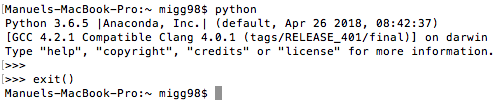
\includegraphics[width=12cm]{./Images/Terminal}
    \label{Terminal}
    \caption{Ejecución y cierre de python desde la terminal.}
\end{figure}

Para abrir archivos de python simplemente ejecutamos el comando para iniciarlo seguido del nombre de nuestro archivo con terminación \textit{.py}.

\section{Jupyter Notebook para análisis de datos}

Python es una lenguaje de programación fácil de aprender y bastante útil para el análisis de datos, y es así que surgen los cuadernillos de trabajo, entre ellos tenemos el creado por Project Jupyter, el Jupyter Notebook.

Para comenzar a trabajar con este cuadernillo es necesario ir a la dirección donde se encuentran los archivos que usaremos en nuestro código (archivos de texto, imágenes, datos numéricos, etc) desde la terminal, posteriormente escribir el comando \textbf{juyter notebook}, al hacer esto se genera un link, el cual se muestra en nuestro navegador, dándonos acceso al cuadernillo de trabajo donde podremos hacer uso de Python y ciertas facilidades que proporciona Jupyter Notebook.

Comenzamos creando un archivo de \textbf{Python3} desde la interfaz de Jupyter, esto nos genera nuestro cuadernillo donde lo primero que veremos será un bloque de código. La ventaja de usar Jupyter es la implentación de las sugerencias al introducir un comando, el autocompletado de aquello que escribimos, la interfaz que presenta, la visualización de la información que estamos manejando y generando, entre otras.

\subsection{Autocompletado}

Una función interesante es el \textbf{autocompletado}, basta con simplemente usar la tecla \textbf{TAB} para que se despliegue una lista de opciones con comando del sistema y/o variables creadas durante el programa.

\begin{figure}[h!]
	\center
	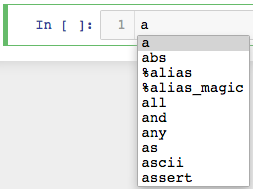
\includegraphics[scale=.5]{./Images/Tabcomplete}
	\label{Tab Complete}
	\caption{Autocompletado usando la tecla TAB.}
\end{figure}

\subsection{Introspección}

La función de \textbf{introspección} permite al usuario conocer información acerca de la función o variable en cuestión. Para hacer uso de esto es necesario agregar un signo de interrogación (\textbf{?}) al principio o al final del objeto por analizar (Figura \ref{fig:Inter}).

\begin{figure}[h!]
	\center
	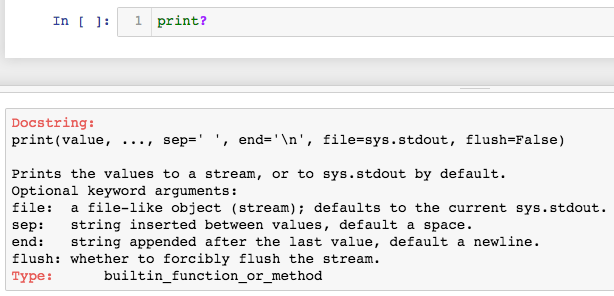
\includegraphics[scale=.4]{./Images/Introspeccion}
	\caption{\label{fig:Inter}Agregando '?' a un objeto brinda información extra.}
\end{figure}

\subsection{Atajos de teclado para la terminal}

Para mejorar la interacción entre el usuario y la interfaz del cuadernillo de trabajo también se cuenta con algunas combinaciones de teclas que permiten desplazarnos, eliminar, agregar, editar o manejar de diversas formas nuestro código. Existen diversos combinaciones para ello pero en el presente trabajo mostraremos sólo algunas de ellas (Figura \ref{fig:Atajos}).

\begin{figure}[h!]
	\center
	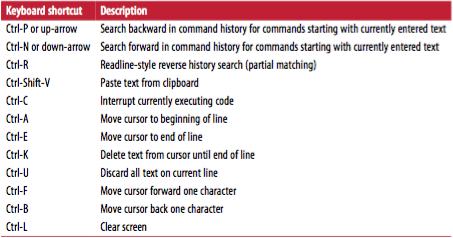
\includegraphics[scale=.6]{./Images/Atajos}
	\caption{\label{fig:Atajos}Atajos desde el teclado (Wes McKinney).}
\end{figure}

\subsection{Comandos mágicos}

Otra característica interesante son los comandos "mágicos", estos son una serie de comandos especiales los cuales facilitan tareas comunes y permiten tomar control del comportamiento del sistema. Entre los comandos tenemos uno de los más destacados para hacer gráficas, el comando \textbf{\%matplotlib inline}. Este comando permite generar gráficas dentro del cuadernillo de trabajo, además de evitar que la gráfica interfiera en la sesión de la consola.

Al igual que con los atajos para la terminal, tenemos una variedad de opciones para los comandos mágicos y existen muchas otras usando \textbf{\%magic}. En la figura \ref{fig:magic} vemos algunos ejemplos de ello.

%\pagebreak

\begin{figure}[h!]
	\center
	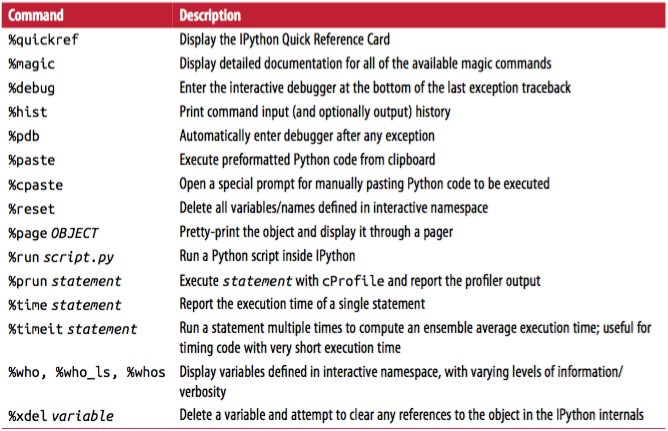
\includegraphics[scale=.35]{./Images/Magic_Table}
	\caption{\label{fig:magic}Algunos de los comandos mágicos disponibles (Wes McKinney).}
\end{figure}

\section{Básicos del lenguaje Python}

A continuación se presentarán algunos aspectos básicos del lenguaje Python con los cuales podremos comenzar a crear nuestros propios códigos y comprender otros que nos parezcan interesantes en Internet. Los aspectos a ver incluyen la semántica del lenguaje, los formatos y el control de flujo de un programa.

\subsection{Semántica del lenguaje}

\begin{description}
\item[Indentación, no llaves].
\newline A diferencia de muchos otros lenguajes de programación, Python hace uso de la indentación, la cual consiste en los espacios o las tabulaciones que le apliquemos al código para separarlo y estructurarlo. De esta manera al realizar nuestro código resultará más sencillo leerlo y que otros también lo hagan.

\item[Todo es un objeto].
\newline Otra característica importante en Python es su \textit{modelo de objeto}, esto consiste en el hecho de que cada número, carácter, estructura de datos, función, clase, modulo y demás es un objeto dentro del lenguaje de Python. Cada objeto tiene un tipo e información interna. Este hecho hace que Python sea un lenguaje bastante flexible.

\item[Comentarios].
\newline Para agregar comentarios en Python es necesario utilizar el gato (\#) antes de la línea de código que deseemos omitir pues todo lo que se encuentre a la derecha del \# será ignorado. Esta es una manera sencilla y útil de hacer comentarios o inhabilitar comandos sin borrarlos, de esta manera podríamos utilizarlos nuevamente después.

\item[Llamando funciones y objetos].
\newline Para llamar a las funciones basta con agregar un par de paréntesis al final y agregar un cero o más argumentos, también es posible asignar el resultado de alguna función a una variable y, dado que son objetos, es posible aplicarle funciones internas que permiten al usuario conocer información específica acerca de ellas (Véase la figura \ref{fig:funcion}).

\begin{figure}[h!]
	\center
	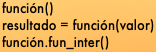
\includegraphics[scale=.8]{./Images/Funcion}
	\caption{\label{fig:funcion} Algunas opciones con una función.}
\end{figure}

\item[Traspaso de variables y argumentos].
\newline Cuando le asignamos una variable (o nombre) a un elemento, lo que estamos haciendo es crear una referencia a él mismo. Tomemos como ejemplo una variable \textbf{A} con los valores 1, 2 y 3. \newline

\begin{center}
	\textbf{A = [1, 2, 3]}
\end{center}

Posteriormente igualamos \textbf{A} con otra variable \textbf{B}.

\begin{center}
	\textbf{B = A}
\end{center}

Dado que ambas variables son una referencia a la lista de valores, si a \textbf{A} le agregamos el valor de 4, \textbf{B} también lo tendrá.

\begin{center}
	\textbf{a.append(4)}

	\textbf{b = [1, 2, 3, 4]}
\end{center}

\item[Atributos y métodos].
\newline Los objetos en Python tiene atributos (otros objetos de Python "dentro" de los objetos) y métodos (funciones asociadas a los objetos que pueden acceder a la información interna del objeto), para acceder a estas funciones simplemente debemos de escribir el nombre de la variable, seguido de un punto '.' y presionamos la tecla \textbf{TAB} para ver sus opciones (Véase la figura \ref{fig:atributos}).

\begin{figure}[h!]
	\center
	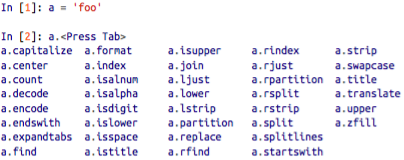
\includegraphics[scale=.7]{./Images/atributos}
	\caption{\label{fig:atributos} Atributos para una cadena de caracteres.}
\end{figure}

\item[Importando].
\newline En Python un modulo puede ser cualquier archivo que cuente con la extensión \textit{.py} y contenga un código de Python. Para acceder a todo su contenido es necesario importarlos a nuestro código.

\begin{center}
	\textbf{import nombre-modulo as n-m} (abreviación del modulo)
\end{center}

Y posteriormente podemos llamar alguna función, variable o lo que deseemos del modulo usando la siguiente sintaxis.

\begin{center}
	\textbf{n-m . nombre-variable-o-funcion()} (nombres unidos por el .)
\end{center}

\item[Operadores binarios y comparaciones].
\newline La mayoría de los operadores binarios y de comparación son como lo esperaría cualquier persona. Existen una lista completa con los operadores que podemos trabajar (Véase la figura \ref{fig:operador}).

\begin{figure}[h!]
	\center
	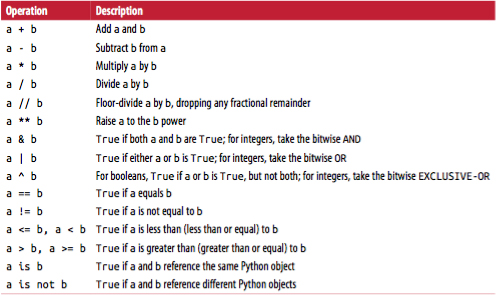
\includegraphics[scale=.65]{./Images/operadores}
	\caption{\label{fig:operador} Operadores disponibles en Python (Wes McKinney).}
\end{figure}

\end{description}

\subsection{Tipo escalar}

Dentro del lenguaje Python existen ciertos tipos en para manejar la información numérica, cadenas de caracteres, valores booleanos y fechas y horas. Todos estos valores usualmente son llamados tipos escalares (Vease la figura \ref{fig:tipos}).

\begin{figure}[h!]
	\center
	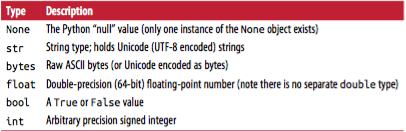
\includegraphics[scale=.68]{./Images/tipos}
	\caption{\label{fig:tipos} Tipos existentes en Python.}
\end{figure}

\begin{description}
\item[Tipos numéricos].
\\ Los tipos primarios para números en Python son \textbf{int} y \textbf{float}. Los números del tipo \textbf{int} pueden almacenar números arbitrariamente grandes. Por otro lado, los números de punto flotante son el tipo \textbf{float} y pueden expresarse con notación científica. \pagebreak

Finalmente, cuando hagamos divisiones existen dos tipos de resultados posibles; al dividir dos números enteros, el resultado puede no ser entero, es entonces cuando se generar un número del tipo \textbf{float}.

\begin{center}
	\textbf{Entrada:} 3/2 (Números \textbf{int})
	
	\textbf{Salida:} 1.5 (Número \textbf{float})
\end{center}

Sin embargo, si deseamos que el resultado se mantenga siendo un número del tipo \textbf{int} debemos agregar una diagonal (/) más a la operación.

\begin{center}
	\textbf{Entrada:} 3//2 (Números \textbf{int})

	\textbf{Salida:} 1 (Número \textbf{int})	
\end{center}

\item[Cadenas de caracteres].
\\ Para crear una variable que contenga caracteres debemos de usar las comillas sencillas (') o dobles (") al principio y fin de los caracteres que deseamos almacenar; mientras que para almacenar caracteres en distintos renglones hacemos uso de tres comillas sencillas o dobles de igual modo que para un solo renglón.
\\ Las cadenas de caracteres no son modificables pues una vez creada la variable no será posible alterar su contenido pero sí es posible convertir diversos objetos de Python en una cadena de caracteres usando la función de \textbf{str}.

{\raggedright 
\textbf{Entrada 1:} A = 5.6 (A es del tipo \textbf{int}) \\
\textbf{Entrada 2:} S = str(A) (S recibe A como una cadena de caracteres) \\
\textbf{Entrada 3:} print(S) \\
\textbf{Salida 3:} 5.6 (El valor es ahora una cadena de caracteres)}

\item[Booleanos]. \\
Los únicos dos valores son \textbf{True} y \textbf{False}. Las comparaciones y otras expresiones condicionales al ser evaluadas arrojan uno de estos dos valores. Estos valores están relacionados con las funciones lógicas \textbf{and} y \textbf{or}.

\item[Fecha y hora]. \\
El modulo \textbf{datetime} de Python incluye tres tipos de objetos: (1) \textbf{datetime}, el tipo más usado de los tres, (2) \textbf{date}, utilizado para almacenar alguna fecha y (3) \textbf{time}, que almacena únicamente datos con formato de hora. Usualmente es más usado el tipo \textbf{datetime} ya que es posible usar un \textit{método} (función interna del objeto) para tomar el valor de la fecha u hora, siempre y cuando cumpla con un formato reconocible (Véase la figura \ref{fig:formatos}).

\begin{figure}[h!]
	\center
	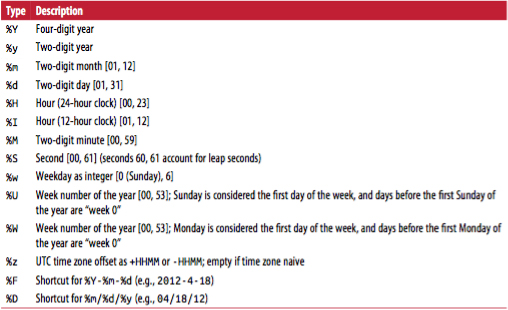
\includegraphics[scale=.65]{./Images/formatos}
	\caption{\label{fig:formatos} Formatos disponibles para el tipo \textbf{datetime} (Wes McKinney).}
\end{figure}

\end{description}

\subsection{Control de flujo}
Python tiene sus palabras clave para referirse a ciertas condiciones lógicas, bucles y otros conceptos para controlar el flujo del programa. A continuación veremos más acerca de esto.

\begin{description}
\item[If, else if y else]. \\
La declaración de un \textbf{if} es una de las más comunes y al igual que en otros lenguajes lo que hace este comando es evaluar si la condición dada es verdadera y proceder a realizar la tarea que sea asignada para este caso o de igual manera evaluar otras situaciones hasta que la condición se cumpla, o no, para proceder. Se pueden agregar tantas condiciones/situaciones como se deseen, solamente se debe agregar el comando \textbf{elif} para cada una de esas condiciones extras.

\begin{center}
	\textbf{if} \textit{condicion-1} \textbf{:} \\
	\hspace{1em} \textit{accion-1} \\
	\textbf{elif} \textit{condicion-2} \textbf{:} \\
	\hspace{1em} \textit{accion-2} \\
	\textbf{else} \textit{condicion-3} \textbf{:} \\
	\hspace{1em} \textit{accion-3}
\end{center}

\item[For loops]. \\
Este controlador se utiliza para llevar a cabo un proceso cierta cantidad de veces, modificando el valor de una variable dada hasta cumplir con la secuencia a seguir, haciendo que el proceso dado sea automatizado. La sintaxis es la siguiente:

\begin{center}
	\textbf{for} \textit{variable} \textbf{in} \textit{secuencia} \textbf{:} \\
	\textit{accion-a-realizar}
\end{center}

También es posible agregar un comando \textbf{break} dentro de este controlador y sirve para salir del proceso cuando se cumpla cierta condición que sea establecida en el código.

\item[While loops]. \\
El presente comando es parecido al visto anteriormente pues realizar un proceso iterativo, salvo que en esta ocasión la cantidad de veces que se ejecute la acción indicada depende de una condición lógica, y mientras esta dé como resultado verdadero (\textbf{True}), las iteraciones seguirán hasta que el resultado sea lo contrario.

\begin{center}
	\textbf{while} \textit{condicion-logica} \textbf{:} \\
	\textit{accion}
\end{center}

\item[Pass]. \\
Este comando (\textbf{pass}) es un auxiliar más (al igual que el \textbf{break}) pero con la diferencia que al utilizarlo el proceso no es interrumpido sino que más bien simplemente se ignora está opción y se procede de forma habitual en el código.

\item[Range]. \\
El comando es utilizado para crear un iterador que sigue una secuencia de números enteros igualmente espaciados. Para crearlo es simplemente necesario insertar el número hasta el cual se generará, siendo de este modo el predeterminado (comenzando desde 0 y aumentando en 1 el valor del iterador), o bien, es posible indicar en qué número comienza, en cuál termina y el incremento que se recibirá).

\begin{center}
	\textbf{range(}\textit{valor-inicial}\textbf{,} \textit{valor-final}\textbf{,} \textit{aumento}\textbf{)}
\end{center}

\end{description}

\begin{thebibliography}{1}
\bibitem{1} Wes McKinney, \textit{Python for Data Analysis. Data Wrangling with Pandas, NumPy, and IPhyton}, second edition, O'Reilly, (2017).
\end{thebibliography}

\end{document}
